\chapter{The Slip}

\vspace{1em}
\hfill
\begin{minipage}[c]{0.55\textwidth}
\raggedleft
\small\itshape
It from bit. Every it derives its function, its meaning, its very existence from the apparatus-elicited answers to yes-or-no questions.\\[0.5em]
\upshape\footnotesize John Archibald Wheeler, ``Information, Physics, Quantum'' (1990)
\end{minipage}%
\hspace{0.5em}
\begin{minipage}[c]{0.12\textwidth}
% \includegraphics[width=\textwidth]{figures/ch06_slip.png}
\end{minipage}
\vspace{1.5em}

\noindent Chapter 5 ended with a small phrase. \emph{What remains is interpretation.} This chapter takes the first step the mathematics does not force.

So far, the universal prior $M$ has been a distribution on hypotheses. A way of weighting candidate explanations of the data you have. A prior over the theories you might hold about the world.

The step is to read $M$ differently. Not as a measure over what you might believe. As a measure over what is.

\section*{Two readings}

The equation $M(x) = \sum_{p\,:\,U(p) = x*} 2^{-|p|}$ does not say what $M(x)$ \emph{means}. It says how to compute it. Two interpretations are available, and they are not the same thing.

The first reading is epistemic. $M(x)$ is the probability that a careful reasoner should assign to observing $x$, given no prior data. The universal prior describes optimal belief. It tells the agent how to weight her hypotheses about the world. Nothing in this reading commits to anything about the world itself; the universal prior is a fact about reasoning, not about reality.

The second reading is ontic. $M(x)$ is the measure of \emph{realities} that produce $x$. The universal prior describes the frequency with which $x$ appears among the things that exist. Under this reading, $M$ is a fact about reality, not about reasoning.

The mathematics is the same. The metaphysical commitment is different.

\begin{figure}[h]
\centering
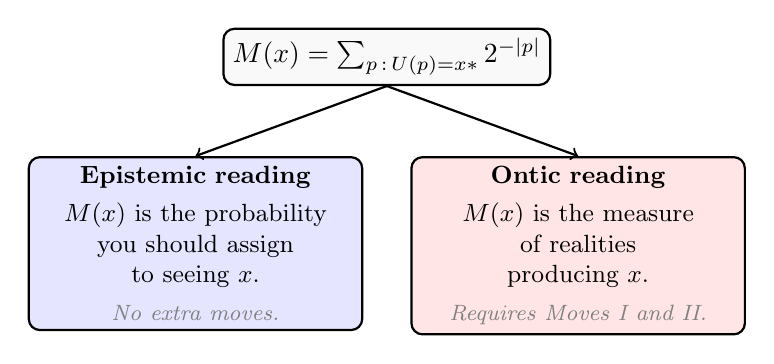
\begin{tikzpicture}[scale=0.9]
  % Top: the equation
  \node[draw, thick, rounded corners, fill=gray!5, font=\normalsize] (top) at (5, 5) {$M(x) = \sum_{p\,:\,U(p) = x*} 2^{-|p|}$};

  % Left box: epistemic
  \node[draw, thick, fill=blue!10, rounded corners, font=\small, text width=4cm, align=center, anchor=north] (left) at (2.3, 3.6) {\textbf{Epistemic reading} \\[0.3em] $M(x)$ is the probability \\you should assign \\to seeing $x$. \\[0.3em] \footnotesize\itshape\textcolor{gray}{No extra moves.}};

  % Right box: ontic
  \node[draw, thick, fill=red!10, rounded corners, font=\small, text width=4cm, align=center, anchor=north] (right) at (7.7, 3.6) {\textbf{Ontic reading} \\[0.3em] $M(x)$ is the measure \\of realities \\producing $x$. \\[0.3em] \footnotesize\itshape\textcolor{gray}{Requires Moves I and II.}};

  % Arrows
  \draw[->, thick] (top.south) -- (left.north);
  \draw[->, thick] (top.south) -- (right.north);
\end{tikzpicture}
\caption{The slip. The same equation, $M(x)$, can be read in two ways. The epistemic reading needs only the bedrock from Part I. The ontic reading requires two further commitments, labeled Move I and Move II below. This chapter takes the ontic reading and tracks what each commitment costs.}
\label{fig:slip}
\end{figure}

This chapter takes the second reading. The next two sections label the moves the second reading requires.

\section*{Move I: Church-Turing applied to reality}

The first commitment.

The Church-Turing thesis, stated for algorithms: any function that can be computed by an effective procedure can be computed by a Turing machine. This is settled. Every reasonable model of computation has been shown equivalent to the Turing machine. Ninety years of testing, no counterexamples.

Move I extends this from algorithms to physics: \emph{any function physically computable by any physical process can be computed by a Turing machine}. The world is computable. The laws of nature are algorithmic.

This is not the original Church-Turing thesis. It is the \emph{physical} Church-Turing thesis, and it is not provable in the same way the original is. It is a claim about what physics is doing. If the laws of nature involve genuinely uncomputable processes (real-valued precision in a load-bearing way, oracle-like cosmological constants, closed timelike curves with continuous parameters), Move I fails.

What Move I buys. The bedrock applies to reality, not just to hypotheses. The universal prior is the right prior over the physical world, not just over an agent's mental world. The dominance theorem says optimal learning catches up to whatever the world is doing, when the world is computable. Move I says: the world is computable, so the theorem applies.

What Move I costs. A substantive metaphysical position. Most physicists accept Move I implicitly, few defend it explicitly. The acceptance is reasonable but provisional. If a robust experimental demonstration of uncomputable physics surfaces, Move I dies, and with it the right to apply the universal prior to reality.

The empirical case for Move I is stronger than its provisional status suggests. Every physical process humans have measured has fallen within the Turing-computable class. Every theoretical framework that has survived experimental test, from Newtonian mechanics through quantum field theory, fits inside that class. The negative claim, that physics involves some genuinely uncomputable process in a load-bearing way, has no experimental support. The default empirical position is Move I. Refusing it requires positive evidence, not just possibility.

The book takes Move I. It labels it.

\section*{Move II: The Library is real}

The second commitment.

Move I makes the universal prior applicable to reality. It is the right prior over computable physical processes. But \emph{which} computable physical process?

The naive answer: the one we inhabit. There is one world; the universal prior tells us how to reason about it.

Move II is the stronger answer. The universal prior is not a measure on one world. It is a measure on \emph{all} computable structures. The Library of Babel from Chapter 2 is not a metaphor. It is the ontological substrate. Every entry in the Library corresponds to a real structure. Every program, when interpreted as describing a universe, produces a real history.

This is the \emph{Computable Universe Hypothesis} (CUH). Its unrestricted cousin, Tegmark's Mathematical Universe Hypothesis, says all mathematical structures exist. CUH restricts that claim to the computable ones, which is what makes the ontology well-defined and the measure (the universal prior) natural. Mathematical structures that are not computable, if there are any in the load-bearing sense, are not in the Library.

What Move II buys. A natural account of why we observe a simple universe. Observers in low-$K$ universes have higher measure under the universal prior. We expect to find ourselves in a universe with short laws, because that is where the measure concentrates. The simplicity bias becomes ontologically grounded rather than epistemically chosen.

It also buys multiplicity. The Library contains many universes consistent with any partial data. Your observations restrict you to a subset of the Library; the measure on that subset describes which universe is yours, weighted by frequency.

What Move II costs. A vastly larger ontology than ordinary realism. Realities you do not inhabit are as real as the one you do. The version of you that turned left at the bakery this morning exists at her coordinates, in her universe, with her structure. So does the version that turned right. So does the version that did not exist at all because the bakery had a different owner whose daughter never met yours.

This is more than most metaphysical positions ask. The book takes Move II.

It is worth asking, before going further, which of the two ontologies on the table is the informationally more demanding one. The standard intuition is that CUH is the more demanding position. The chapter's tools suggest the answer is the other one.

\section*{Information is in the cut}

The standard objection to the Computable Universe Hypothesis: it multiplies entities. By declaring vast numbers of realities to exist, it inflates the ontology far beyond the one universe we observe. Occam's razor, the usual simplicity heuristic, seems to forbid such inflation. \emph{Do not multiply entities beyond necessity.}

The objection rests on a confusion the Library makes visible.

Chapter 2 established that informational cost lives in the cut, not in the totality. The empty set is cheap. The universal set is cheap. Both are describable in a phrase. The interesting subsets, the ones that require selecting some elements from a larger possibility space, are where description length lives.

Apply the principle to ontology. Two competing positions on what exists.

\begin{figure}[h]
\centering
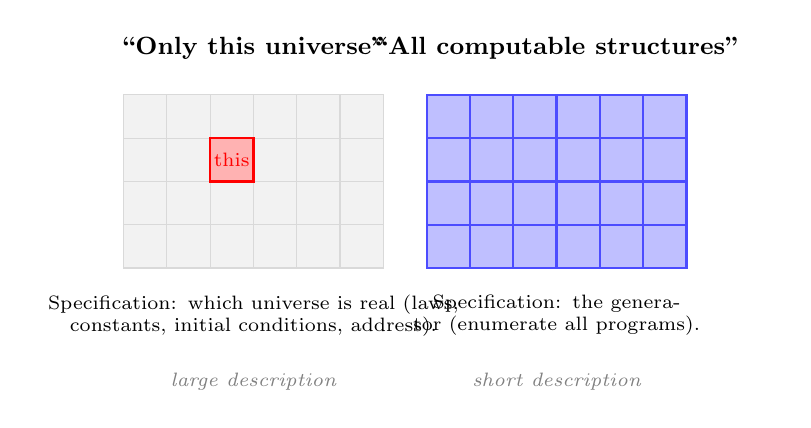
\begin{tikzpicture}[scale=0.55]
  % LEFT: Only this universe
  \node[font=\small\bfseries, anchor=south] at (3, 4.6) {``Only this universe''};

  % Faded grid of universes (Library, mostly grayed)
  \foreach \x in {0,1,2,3,4,5} {
    \foreach \y in {0,1,2,3} {
      \draw[gray!30, fill=gray!10] (\x, \y) rectangle ({\x+1}, {\y+1});
    }
  }
  % One highlighted universe
  \draw[thick, red, fill=red!30] (2, 2) rectangle (3, 3);
  \node[font=\scriptsize, red] at (2.5, 2.5) {this};

  % Label below
  \node[font=\scriptsize, anchor=north, text width=5.5cm, align=center] at (3, -0.4) {Specification: which universe is real (laws, constants, initial conditions, address).};
  \node[font=\scriptsize\itshape, anchor=north, gray] at (3, -2.2) {large description};

  % RIGHT: All computable structures
  \node[font=\small\bfseries, anchor=south] at (10, 4.6) {``All computable structures''};

  % Fully lit grid
  \foreach \x in {7,8,9,10,11,12} {
    \foreach \y in {0,1,2,3} {
      \draw[thick, blue!70, fill=blue!25] (\x, \y) rectangle ({\x+1}, {\y+1});
    }
  }

  % Label below
  \node[font=\scriptsize, anchor=north, text width=5.5cm, align=center] at (10, -0.4) {Specification: the generator (enumerate all programs).};
  \node[font=\scriptsize\itshape, anchor=north, gray] at (10, -2.2) {short description};
\end{tikzpicture}
\caption{Two ontologies side by side. The single-universe view (left) requires specifying \emph{which} universe is real: a cut from the Library that takes information proportional to the description length of our particular universe. The CUH view (right) requires only the generator, which is a few lines. By description length, the second is the informationally simpler ontology.}
\label{fig:cut-argument}
\end{figure}

\emph{Position One: only this universe exists.} To assert this position, one must specify which universe is real. The specification is a long string. It must include the laws of dynamics, the values of every physical constant, the initial conditions of the universe, and the address of our universe within the Library of all possibilities. The information cost is the Kolmogorov complexity of our particular universe, which is large.

\emph{Position Two: all computable structures exist.} To assert this position, one must specify the generator. The generator is a few lines of pseudocode: \emph{enumerate all programs of increasing length, and let each compute its output}.\footnote{``Generator'' is metaphor. The Library is not produced by an algorithm running in time; it is a static object, the set of all programs runnable on a universal Turing machine. The few lines of pseudocode are our way of indexing the Library, not its constitution. This mirrors the treatment of physical spacetime in \textit{Worldlines}: a static four-dimensional manifold that we traverse via our worldlines. The Library, like the manifold, is timeless. Our use of words like ``generation'' reflects how we encounter the Library, not what it is.} The information cost is the description length of the generator, which is small.\footnote{The generator's own description is a bit string of finite length, so it is itself one of the programs in the enumeration. The Library contains its own description. In Move II's reading, the universe containing the algorithm that enumerates all universes is also in the Library. The self-reference is structural and harmless.}

By description length, the second position is the simpler ontology. The first specifies which universe is real; the second specifies nothing beyond the rule that generates the Library.

This does not prove Move II. Applying a description-length principle to existence itself is a further step the bedrock does not force, and simplicity is one input among many to a metaphysical commitment. But the dialectic is reframed. The intuition that ``just one world'' is simpler is, by the cut principle, backwards. The single-universe view requires more information to specify, not less.

The book takes Move II partly for this reason. It is the move that requires the least cut.

\section*{Where this leaves you}

The slip has been made. The universal prior, which started as a way to weight hypotheses, is now a way to weight realities. The Library has been read ontologically.

The picture this gives, the older question it sharpens, and the limits of any of it are the subjects of the next chapter.
